\documentclass[a4paper]{article}


\usepackage{geometry}
\geometry{legalpaper, margin=1.28in}


\usepackage[english]{babel}
\usepackage[utf8]{inputenc}
\usepackage{amsmath}
\usepackage{graphicx}
\usepackage[colorinlistoftodos]{todonotes}

\title{Model-based Design for Closed-loop Medical Devices}

\author{Zhihao Jiang}

% \date{\today}

\begin{document}
\maketitle

% \begin{abstract}
% Your abstract.
% \end{abstract}

\section*{Thesis Problem}
Closed-loop medical devices like implantable pacemakers have both therapeutic and diagnostic capabilities, which are performed by increasingly sophisticated software component. 
The safety and efficacy of closed-loop medical devices can only be evaluated within their physiological contexts. 
However, currently the only closed-loop validation method for medical devices is clinical trial on real patients, which is costly and pose significant risks on the patients participating in the trial. 
There is urgent need to identify potential safety violations earlier during the software design process.

\section*{Thesis Statement}
In this thesis, I propose to use model-based design throughout the software design process of closed-loop medical devices. 
By applying model-based techniques including model abstraction, model checking, model translation, closed-loop validation of the device software can be performed during different steps of the software design process.
The results of these closed-loop validation provide safety and efficacy evidence of the device software, which are also compatible with the current regulation framework. 
Applying the proposed model-based techniques can potentially reduce the time and money cost during the software development for all parties involved, including device manufacturers, the regulation agency and also the physicians.

\section*{Thesis Summary}
In this thesis, I propose a model-based design framework for closed-loop validation of closed-loop medical devices, and use implantable cardiac devices as case study. 
Model-based closed-loop evaluation of medical devices require models of the physiological conditions of the patient(s) that can interact with the device model in closed-loop. 
In this thesis I developed a heart model structure which can be used to simulate electrical activities of the heart for various heart conditions.
The model structure is capable of generating synthetic signals that can be used as inputs to implantable cardiac devices, and also able to respond to device outputs. 
The model structure was validated by the physicians for capable of generating physiological-relevant signals for variety of heart conditions.
Variations of the heart model structure can be used for closed-loop evaluation of the device in different activities during the software development process. 
The heart model is also available on hardware platform to interact with an actual device in closed-loop.

%The first step in the model-based design framework is risk analysis on abstract model of the device using closed-loop model checking technique.
Early in the software design process, risk analysis can be performed on abstract model of the device using closed-loop model checking.
An abstract model of the device, and heart models representing different heart conditions are modeled with timed-automata formalism in model checker UPPAAL.
Safety risks of the devices are specified as properties and the closed-loop model is verified for the existence of safety violations.
The result of the model checking fits seamlessly into the risk analysis activities mandated by the regulator.
The physiological models used for closed-loop model checking should be able to cover all the physiological behaviors specified in the properties and their states should be expressive enough to maintain physiological context. 
Another contribution of this thesis is an abstraction and refinement technique which can balance the coverage and expressiveness of the physiological model during closed-loop model checking.

After the abstract model of the device is validated through model checking, a rigorous process is required to translate the abstract model into the implementation. 
In this thesis I developed a model translation tool to translate UPPAAL timed-automata models to Simulink Stateflow charts.
The Stateflow charts can then be generated into code implementation using Simulink Coder.
The model translation tool ensures that safety requirements validated during model checking are preserved in the implementation.

Another contribution of this thesis is to use heart models to represent virtual patient groups and perform \emph{model-based clinical trials (MBCT)} that can help the planning of an actual clinical trial. 
In this thesis, model-based clinical trials are performed to compare the performance of two implantable cardioverter defibrillators (ICD). 
The result of the MBCTs demonstrates comprehensive insights that match the result of the actual clinical trial, which would increase the chance of a success trial and reduce cost in time and money.

The contributions above incorporate model-based design seamlessly into the existing regulation framework, and can be used to develop safer and cheaper closed-loop medical devices. 
\newpage
\section{Motivation}
Medical devices play an essential role in the care of patients around the world, and can have a life-saving effect.
To cite one example, 
%an estimated 3 million people worldwide have implanted pacemakers (a heart rhythm adjustment device), with \~600,000 added annually.
%Cardiac Pacemakers From the Patient's Perspective circ.ahajournals.org/content/105/18/2136.full
in the US, \~ 800,000 people have an implanted defibrillator (a heart rhythm management device), with 10,000 added monthly.
%http://asktheicd.com/tile/106/english-implantable-cardioverter-defibrillator-icd/how-many-people-have-icds/
Clinical trials have presented evidence that patients implanted with defibrillators have a mortality rate reduced by up to 31\%.
% MADIT II trial
Financially, the medical device market is worth \$289 billion.
%Of that, \$110 billion is in the US alone, with this number projected to reach \$133 billion in 2016.
%http://selectusa.commerce.gov/industry-snapshots/medical-device-industry-united-states
Examples include everything from adhesive bandages to drug infusion pumps, surgical robots, deep brain stimulation systems and devices still undergoing basic research like the artificial pancreas.
%In fact, many device companies are in the no-revenue startup phase, indicating a vigorous research environment.
These are safety-critical technologies combining hardware and software, each of which must be rigorously validated to be efficacious and safe.
\begin{figure}[b]
	\centering
	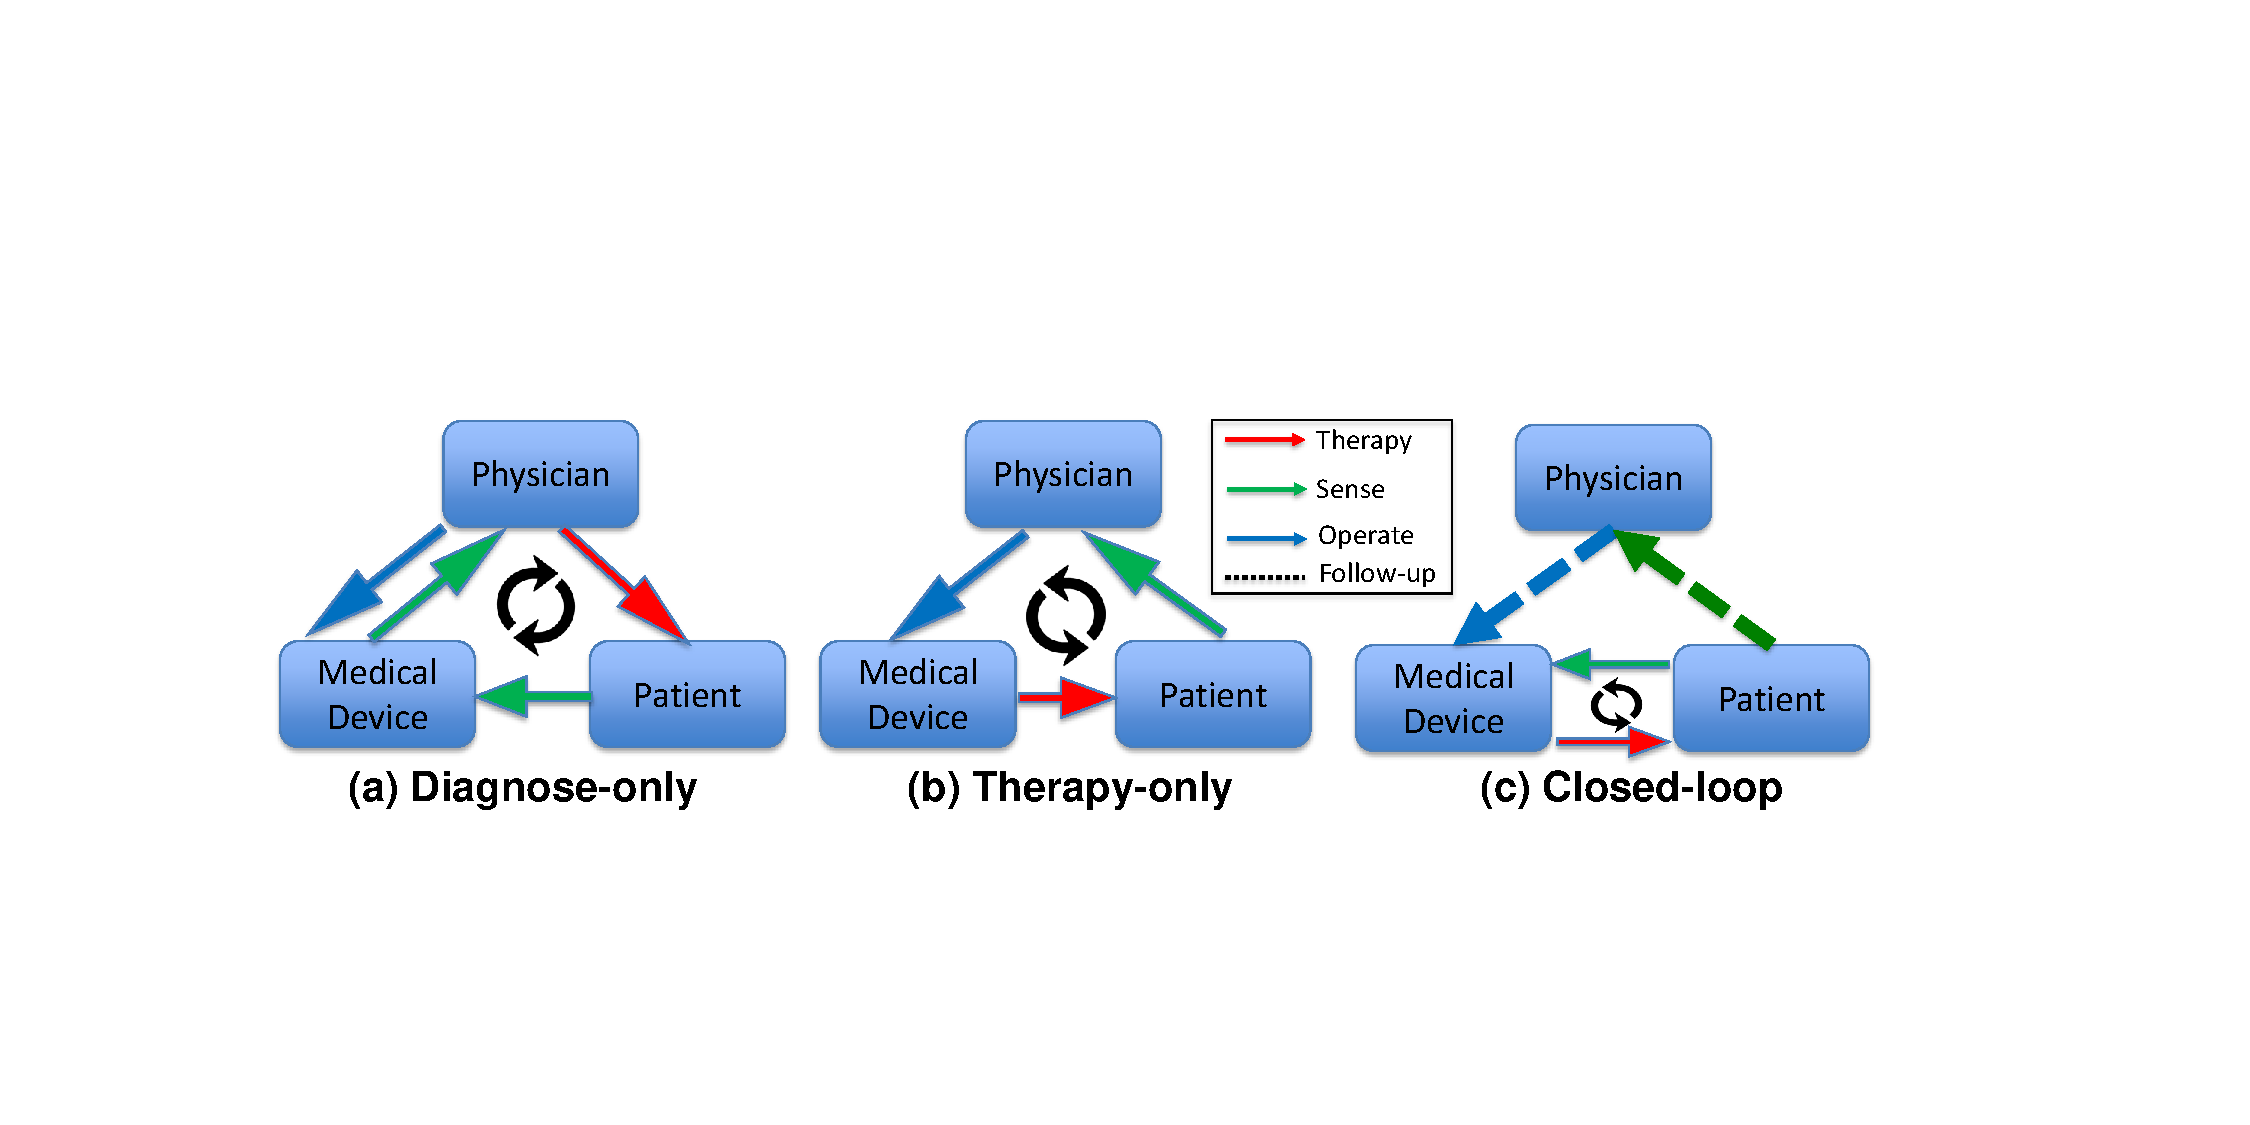
\includegraphics[scale=0.35]{figs/closed-loop.pdf}
	\caption{\small Open-loop and closed-loop medical devices. The open-loop devices has medical professionals in the loop while the closed-loop medical devices interact with patient physiology directly.}
	\label{fig:closed-loop}
\end{figure}

There are two categories of medical devices. 
One category is \emph{open-loop medical device} which has only therapeutic or diagnostic capability, i.e. infusion pumps. 
Open-loop medical devices are normally operated by professional medical care providers, which provides reliable safety guarantees (Fig. \ref{fig:closed-loop}).
On the other hand, there is an emerging category referred to as \emph{closed-loop medical devices}, which has both therapeutic and diagnostic capability.
An example of closed-loop medical devices is implantable pacemaker which diagnoses patient condition through sensed electrogram signals and deliver electrical pacing to maintain appropriate heart rhythm (Fig. \ref{fig:pacemaker}). 
Closed-loop medical devices interact with human physiology directly, and often times without human intervention.
Therefore device failures like inappropriate therapies may result in serious injuries or death of the patient.
As the result, closed-loop medical devices are categorized by the regulation agencies as the highest risk devices.
\begin{figure}[t]
	\centering
	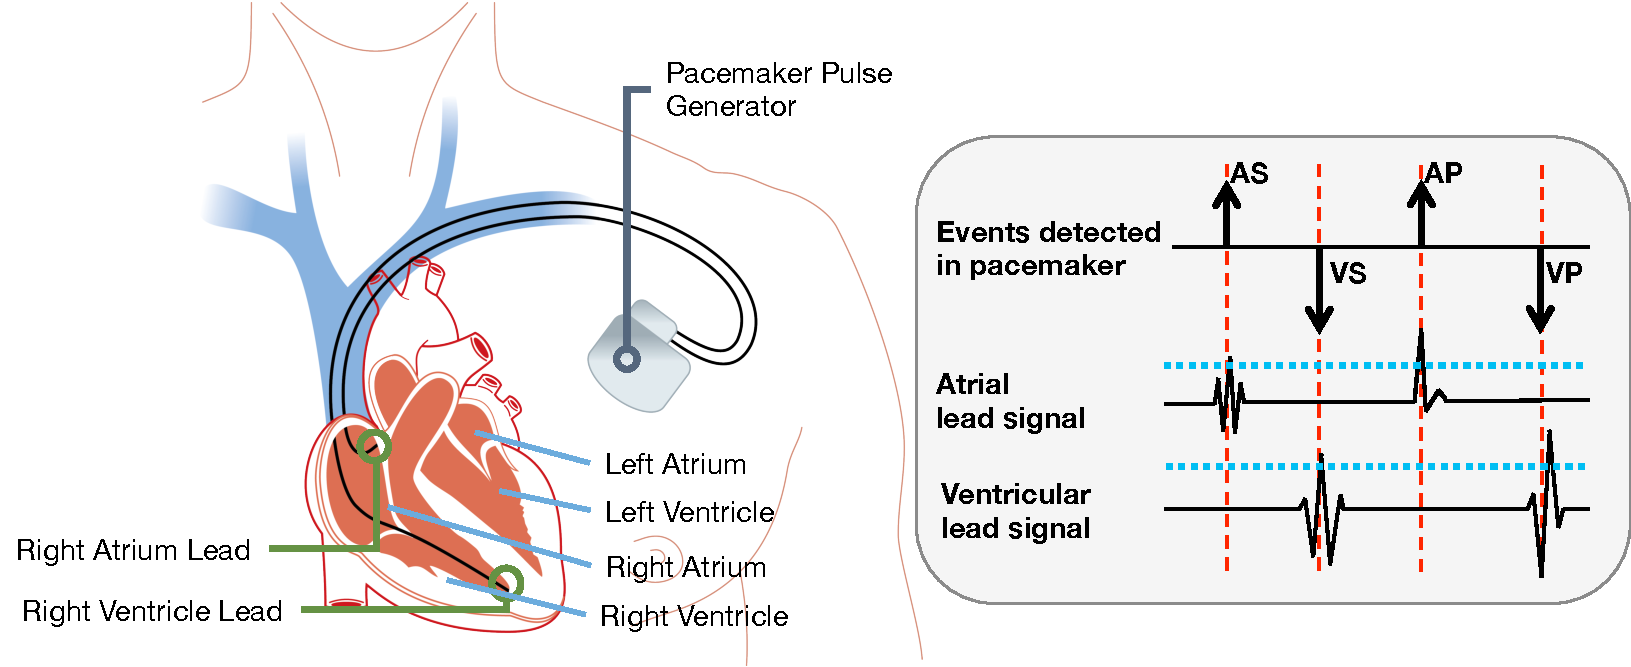
\includegraphics[scale=0.35]{figs/fig1pacemaker.pdf}
	\caption{\small Pacemaker operating in a closed-loop with the heart. The leads sense cardiac electrophysiological activity from inside the heart tissue (AS/VS = Atrial/Ventricular Sense event) and actuate the heart (AP/VP = Atrial/Ventricular Pacing event to maintain a desired heart rate.}
	\label{fig:pacemaker}
\end{figure}
\section{Challenges for Developing Safe Closed-loop Medical Devices}
\subsection{Sophisticated and Unreliable Software}
To guarantee safe operation, closed-loop medical devices need to correctly identify the condition of the patient and deliver appropriate therapy.
The complex run-time diagnoses needed for closed loop performance, and the intricate therapy delivered, has driven most diagnosis and therapy functions into software.
As the algorithms become more sophisticated, more safety issues are related to software design. 
According to the US Food and Drug Administration, in 1996, 10\% of all medical device recalls were caused by software-related issues. 
This percentage rose to an average of 15\% of recalls from 2008 to 2012. 
Implanted cardiac pacemakers and defibrillators have approximately 80,000-100,000 lines of software code which essentially makes all sensing, control and actuation decisions autonomously within the human body, over the 5-7 year device lifetime. 
The primary challenge of high-confidence medical device software is to guarantee the device will never drive the patient into an unsafe condition even though we do not have complete understanding of the physiological plant.  
\subsection{Closed-loop Interaction with Human Physiology}
Closed-loop medical devices directly measure physiological signals from the patient and deliver therapy based on the diagnosis.
The physiology changes its states and corresponding physiological signals in respond to the therapy, therefore the safety and efficacy of the devices have to be validated within its physiological context.
% However, the understanding of human physiology
% Due to the knowledge gap between the domain experts and the software developers, it is impossible to encode 
Currently the only closed-loop validation method is \emph{clinical trials}, in which the performance of the devices are evaluated on real patients.
Clinical trials are costly in terms of time and money, while exposing enrolled patients with risky unproven therapies.
Problems found at this late stage are also very costly to fix.

\begin{figure}[t]
	\centering
	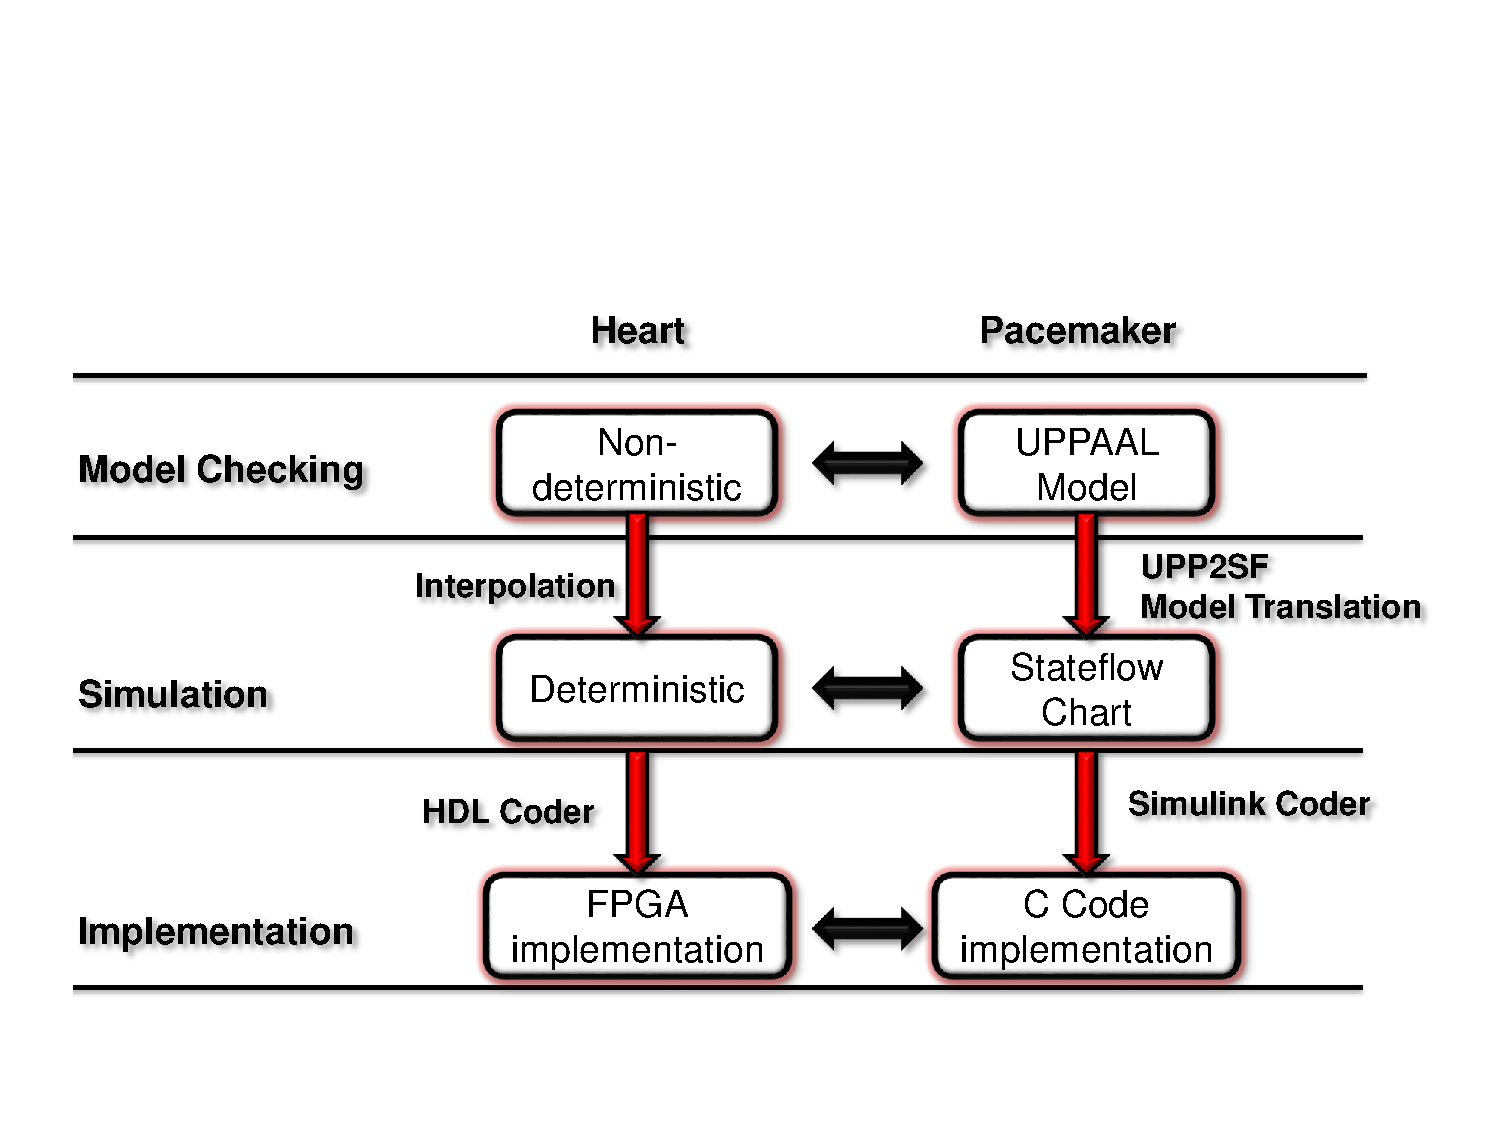
\includegraphics[scale=0.35]{figs/model_based_b.pdf}
	\caption{\small Model-based design of pacemaker software.}
	\label{fig:MBD}
\end{figure}
\section{Proposed Research}
\emph{Model-based Design (MBD)} enables closed-loop validation at earlier design phrase, which can potentially save development cost.
\subsection{Model-based Design Framework}
Fig. \ref{fig:MBD} demonstrates our model-based design framework for implantable pacemaker software.
Throughout the development process we developed heart models to interact with the pacemaker model in closed-loop. 
This framework can potentially be applied for developing other closed-loop medical devices.
There are several key steps within the framework:
\subsection{Physiological Modeling for Closed-loop Device Validation}
In closed-loop MBD, the device (or a model thereof) is connected to a \emph{model} of the ``physiological plant" it interacts with.
%By high confidence verification, researchers mean that under all possible behaviors of the physiological models, the device will act correctly.
The major challenge for model-based closed-loop validation of medical devices is the development of appropriate physiological models.
There are two major differences between modeling physiology and modeling man-made systems:
first, physiology is much more complex and less well-understood than man-made systems like cars and airplanes, and spans several scales from the molecular to the entire human body.
Secondly, the variability between humans is orders of magnitude larger than that between two cars coming off the assembly line.

Different applications of the physiological model have different requirements.
%Using the pacemaker as an example of closed-loop device, and the heart as the organ to be modeled, we present several of the challenges and early results in model-based verification.

\subsection{Risk Analysis with Closed-loop Model Checking}
Risk analysis is an activities mandated by the regulator to provide confidence to the safety of the device, which is currently done manually.
Model checking has been widely used in semi-conductor industry which can check the whole state space of a model for property violations.
By specifying the risks as properties, and model checking the closed-loop model which consists of the device model and a physiological model, we can evaluate whether the risks have been \emph{mitigated}.
With tools like quantitative model checker, we can also evaluate the frequency and severity of the remaining risks.
All of the analysis above can be used as evidence for the safety of the device model.

The major challenge for closed-loop model checking is to develop appropriate physiological models. 
The models should be general enough to cover physiological behaviors from different patient conditions, while at the same time expressive enough to maintain physiological meanings of an execution trace.
There is no single model that can satisfy both requirements and for different properties, different models are required.
It is therefore important to have a rigorous hierachy of physiological models with different abstraction levels and a procedure to choose the appropriate model for a property.
\subsection{Closed-loop Testing}
\subsection{Validated Model to Validated Code}
After the device model has mitigated all the risks, it is essential for the device implementation to preserve those properties.
In our framework, we developed a model translation tool which rigorously translates device model in UPPAAL model checker to Stateflow chart.
The Stateflow chart can then be compiled into C code implementation using Simulink Coder, which completes a tool chain from validated model to validated code.

Due to the limited semantics of the model checking tool, the device model in the model checker is generally an abstraction of the actual device functions.
The biggest challenge for model implementation tool chain is how to deal with the additional behaviors in the actual implementation, and how they affect the property preservation.
\subsection{Model-based Clinical Trials}
%Clinical trials for medical devices are costly in terms of both time and money, therefore they should be carefully planned to reduce the risk of failures.
Currently clinical trials for medical devices are planned with data from previous trials and studies, which do not reflect the current patient population and/or technology advancement.
Clinical trials planned based on these historical data have high chance of failure, which cost a lot of money and time.
Therefore we are proposing \emph{Model-based Clinical Trials (MBCT)}, which use physiological models to generate a virtual patient population and run trials on them to evaluate the performance of the new device.
To clarify, MBCT is not designed to replace clinical trials.
The result of a MBCT can provide useful insights that can be helpful when planning an actual clinical trials.

The validity of MBCT results relies heavily on the validity of the physiological model and the validity of the virtual patient population, which is the biggest challenge for MBCT.

\end{document}